% Options for packages loaded elsewhere
\PassOptionsToPackage{unicode}{hyperref}
\PassOptionsToPackage{hyphens}{url}
\PassOptionsToPackage{dvipsnames,svgnames,x11names}{xcolor}
%
\documentclass[
  letterpaper,
  DIV=11,
  numbers=noendperiod]{scrartcl}

\usepackage{amsmath,amssymb}
\usepackage{iftex}
\ifPDFTeX
  \usepackage[T1]{fontenc}
  \usepackage[utf8]{inputenc}
  \usepackage{textcomp} % provide euro and other symbols
\else % if luatex or xetex
  \usepackage{unicode-math}
  \defaultfontfeatures{Scale=MatchLowercase}
  \defaultfontfeatures[\rmfamily]{Ligatures=TeX,Scale=1}
\fi
\usepackage{lmodern}
\ifPDFTeX\else  
    % xetex/luatex font selection
\fi
% Use upquote if available, for straight quotes in verbatim environments
\IfFileExists{upquote.sty}{\usepackage{upquote}}{}
\IfFileExists{microtype.sty}{% use microtype if available
  \usepackage[]{microtype}
  \UseMicrotypeSet[protrusion]{basicmath} % disable protrusion for tt fonts
}{}
\makeatletter
\@ifundefined{KOMAClassName}{% if non-KOMA class
  \IfFileExists{parskip.sty}{%
    \usepackage{parskip}
  }{% else
    \setlength{\parindent}{0pt}
    \setlength{\parskip}{6pt plus 2pt minus 1pt}}
}{% if KOMA class
  \KOMAoptions{parskip=half}}
\makeatother
\usepackage{xcolor}
\setlength{\emergencystretch}{3em} % prevent overfull lines
\setcounter{secnumdepth}{-\maxdimen} % remove section numbering
% Make \paragraph and \subparagraph free-standing
\ifx\paragraph\undefined\else
  \let\oldparagraph\paragraph
  \renewcommand{\paragraph}[1]{\oldparagraph{#1}\mbox{}}
\fi
\ifx\subparagraph\undefined\else
  \let\oldsubparagraph\subparagraph
  \renewcommand{\subparagraph}[1]{\oldsubparagraph{#1}\mbox{}}
\fi

\usepackage{color}
\usepackage{fancyvrb}
\newcommand{\VerbBar}{|}
\newcommand{\VERB}{\Verb[commandchars=\\\{\}]}
\DefineVerbatimEnvironment{Highlighting}{Verbatim}{commandchars=\\\{\}}
% Add ',fontsize=\small' for more characters per line
\usepackage{framed}
\definecolor{shadecolor}{RGB}{241,243,245}
\newenvironment{Shaded}{\begin{snugshade}}{\end{snugshade}}
\newcommand{\AlertTok}[1]{\textcolor[rgb]{0.68,0.00,0.00}{#1}}
\newcommand{\AnnotationTok}[1]{\textcolor[rgb]{0.37,0.37,0.37}{#1}}
\newcommand{\AttributeTok}[1]{\textcolor[rgb]{0.40,0.45,0.13}{#1}}
\newcommand{\BaseNTok}[1]{\textcolor[rgb]{0.68,0.00,0.00}{#1}}
\newcommand{\BuiltInTok}[1]{\textcolor[rgb]{0.00,0.23,0.31}{#1}}
\newcommand{\CharTok}[1]{\textcolor[rgb]{0.13,0.47,0.30}{#1}}
\newcommand{\CommentTok}[1]{\textcolor[rgb]{0.37,0.37,0.37}{#1}}
\newcommand{\CommentVarTok}[1]{\textcolor[rgb]{0.37,0.37,0.37}{\textit{#1}}}
\newcommand{\ConstantTok}[1]{\textcolor[rgb]{0.56,0.35,0.01}{#1}}
\newcommand{\ControlFlowTok}[1]{\textcolor[rgb]{0.00,0.23,0.31}{#1}}
\newcommand{\DataTypeTok}[1]{\textcolor[rgb]{0.68,0.00,0.00}{#1}}
\newcommand{\DecValTok}[1]{\textcolor[rgb]{0.68,0.00,0.00}{#1}}
\newcommand{\DocumentationTok}[1]{\textcolor[rgb]{0.37,0.37,0.37}{\textit{#1}}}
\newcommand{\ErrorTok}[1]{\textcolor[rgb]{0.68,0.00,0.00}{#1}}
\newcommand{\ExtensionTok}[1]{\textcolor[rgb]{0.00,0.23,0.31}{#1}}
\newcommand{\FloatTok}[1]{\textcolor[rgb]{0.68,0.00,0.00}{#1}}
\newcommand{\FunctionTok}[1]{\textcolor[rgb]{0.28,0.35,0.67}{#1}}
\newcommand{\ImportTok}[1]{\textcolor[rgb]{0.00,0.46,0.62}{#1}}
\newcommand{\InformationTok}[1]{\textcolor[rgb]{0.37,0.37,0.37}{#1}}
\newcommand{\KeywordTok}[1]{\textcolor[rgb]{0.00,0.23,0.31}{#1}}
\newcommand{\NormalTok}[1]{\textcolor[rgb]{0.00,0.23,0.31}{#1}}
\newcommand{\OperatorTok}[1]{\textcolor[rgb]{0.37,0.37,0.37}{#1}}
\newcommand{\OtherTok}[1]{\textcolor[rgb]{0.00,0.23,0.31}{#1}}
\newcommand{\PreprocessorTok}[1]{\textcolor[rgb]{0.68,0.00,0.00}{#1}}
\newcommand{\RegionMarkerTok}[1]{\textcolor[rgb]{0.00,0.23,0.31}{#1}}
\newcommand{\SpecialCharTok}[1]{\textcolor[rgb]{0.37,0.37,0.37}{#1}}
\newcommand{\SpecialStringTok}[1]{\textcolor[rgb]{0.13,0.47,0.30}{#1}}
\newcommand{\StringTok}[1]{\textcolor[rgb]{0.13,0.47,0.30}{#1}}
\newcommand{\VariableTok}[1]{\textcolor[rgb]{0.07,0.07,0.07}{#1}}
\newcommand{\VerbatimStringTok}[1]{\textcolor[rgb]{0.13,0.47,0.30}{#1}}
\newcommand{\WarningTok}[1]{\textcolor[rgb]{0.37,0.37,0.37}{\textit{#1}}}

\providecommand{\tightlist}{%
  \setlength{\itemsep}{0pt}\setlength{\parskip}{0pt}}\usepackage{longtable,booktabs,array}
\usepackage{calc} % for calculating minipage widths
% Correct order of tables after \paragraph or \subparagraph
\usepackage{etoolbox}
\makeatletter
\patchcmd\longtable{\par}{\if@noskipsec\mbox{}\fi\par}{}{}
\makeatother
% Allow footnotes in longtable head/foot
\IfFileExists{footnotehyper.sty}{\usepackage{footnotehyper}}{\usepackage{footnote}}
\makesavenoteenv{longtable}
\usepackage{graphicx}
\makeatletter
\def\maxwidth{\ifdim\Gin@nat@width>\linewidth\linewidth\else\Gin@nat@width\fi}
\def\maxheight{\ifdim\Gin@nat@height>\textheight\textheight\else\Gin@nat@height\fi}
\makeatother
% Scale images if necessary, so that they will not overflow the page
% margins by default, and it is still possible to overwrite the defaults
% using explicit options in \includegraphics[width, height, ...]{}
\setkeys{Gin}{width=\maxwidth,height=\maxheight,keepaspectratio}
% Set default figure placement to htbp
\makeatletter
\def\fps@figure{htbp}
\makeatother

\KOMAoption{captions}{tableheading}
\makeatletter
\makeatother
\makeatletter
\makeatother
\makeatletter
\@ifpackageloaded{caption}{}{\usepackage{caption}}
\AtBeginDocument{%
\ifdefined\contentsname
  \renewcommand*\contentsname{Table of contents}
\else
  \newcommand\contentsname{Table of contents}
\fi
\ifdefined\listfigurename
  \renewcommand*\listfigurename{List of Figures}
\else
  \newcommand\listfigurename{List of Figures}
\fi
\ifdefined\listtablename
  \renewcommand*\listtablename{List of Tables}
\else
  \newcommand\listtablename{List of Tables}
\fi
\ifdefined\figurename
  \renewcommand*\figurename{Figure}
\else
  \newcommand\figurename{Figure}
\fi
\ifdefined\tablename
  \renewcommand*\tablename{Table}
\else
  \newcommand\tablename{Table}
\fi
}
\@ifpackageloaded{float}{}{\usepackage{float}}
\floatstyle{ruled}
\@ifundefined{c@chapter}{\newfloat{codelisting}{h}{lop}}{\newfloat{codelisting}{h}{lop}[chapter]}
\floatname{codelisting}{Listing}
\newcommand*\listoflistings{\listof{codelisting}{List of Listings}}
\makeatother
\makeatletter
\@ifpackageloaded{caption}{}{\usepackage{caption}}
\@ifpackageloaded{subcaption}{}{\usepackage{subcaption}}
\makeatother
\makeatletter
\@ifpackageloaded{tcolorbox}{}{\usepackage[skins,breakable]{tcolorbox}}
\makeatother
\makeatletter
\@ifundefined{shadecolor}{\definecolor{shadecolor}{rgb}{.97, .97, .97}}
\makeatother
\makeatletter
\makeatother
\makeatletter
\makeatother
\ifLuaTeX
  \usepackage{selnolig}  % disable illegal ligatures
\fi
\IfFileExists{bookmark.sty}{\usepackage{bookmark}}{\usepackage{hyperref}}
\IfFileExists{xurl.sty}{\usepackage{xurl}}{} % add URL line breaks if available
\urlstyle{same} % disable monospaced font for URLs
\hypersetup{
  pdftitle={Bayesian statistics and pomp},
  pdfauthor={Qianying (Ruby) Lin; Spencer J. Fox},
  colorlinks=true,
  linkcolor={blue},
  filecolor={Maroon},
  citecolor={Blue},
  urlcolor={Blue},
  pdfcreator={LaTeX via pandoc}}

\title{Bayesian statistics and pomp}
\author{Qianying (Ruby) Lin \and Spencer J. Fox}
\date{}

\begin{document}
\maketitle
\ifdefined\Shaded\renewenvironment{Shaded}{\begin{tcolorbox}[interior hidden, boxrule=0pt, sharp corners, borderline west={3pt}{0pt}{shadecolor}, enhanced, breakable, frame hidden]}{\end{tcolorbox}}\fi

\hypertarget{lecture-outline}{%
\subsection{Lecture outline}\label{lecture-outline}}

\begin{enumerate}
\def\labelenumi{\arabic{enumi}.}
\tightlist
\item
  Motivating Bayesian statistics
\item
  Short introduction to Bayesian statistics and theory
\item
  Introduction to MCMC
\item
  Introduction to PMCMC
\item
  Simple influenza case study
\end{enumerate}

\hypertarget{what-we-have-covered-so-far}{%
\subsection{What we have covered so
far}\label{what-we-have-covered-so-far}}

\Huge

\[p(y|\theta)\]

\Large

\begin{itemize}
\tightlist
\item
  \(y\) can be thought of as your data or observations
\item
  \(\theta\) can be thought of as the model or parameter values
\item
  Called the ``Likelihood''
\end{itemize}

\normalsize

\hypertarget{issues-with-maximum-likelihood-estimation-mle}{%
\subsection{Issues with maximum likelihood estimation
(MLE)}\label{issues-with-maximum-likelihood-estimation-mle}}

\begin{itemize}
\tightlist
\item
  Assumes results occur with some given ``frequency'' over period time
  or replicates/repeated experiments

  \begin{itemize}
  \tightlist
  \item
    If we had the same outbreak hundreds of time, what proportion of
    them would provide confidence intervals that contain the true value
    for the \(R_0\)
  \end{itemize}
\item
  Some difficulties in constraining parameter values based on outside
  data, information, or expert opinion
\item
  Just not really intuitive\ldots{}

  \begin{itemize}
  \tightlist
  \item
    We typically want to say something about the parameters based on the
    data, \(p(\theta|y)\)
  \end{itemize}
\end{itemize}

\hypertarget{bayesian-statistics}{%
\subsection{Bayesian statistics}\label{bayesian-statistics}}

\begin{itemize}
\tightlist
\item
  Bayes theorem provides an intuitive framework to update parameter
  estimates based on both prior knowledge and experimental data
\item
  End result is a posterior distribution, \(p(\theta|y)\), directly
  describing the parameter and model of interest
\item
  Easy to communicate results

  \begin{itemize}
  \tightlist
  \item
    ``The reproduction number is estimated to be x, with a 95\% credible
    interval from y to z''
  \end{itemize}
\item
  Issues

  \begin{itemize}
  \tightlist
  \item
    Computationally expensive
  \item
    Without enough data, prior can bias posterior distribution, but this
    is what you want!
  \end{itemize}
\end{itemize}

\hypertarget{bayes-theorem-1}{%
\subsection{Bayes theorem 1}\label{bayes-theorem-1}}

\Huge

\[p(\theta|y) = \frac{p(y|\theta)p(\theta)}{p(y)}\]

\Large

\begin{itemize}
\tightlist
\item
  \(p(\theta|y)\) is the posterior distribution
\item
  \(p(y|\theta)\) is the likelihood
\item
  \(p(\theta)\) is the prior distribution
\item
  \(p(y)\) is the marginal distribution (sometimes called a normalizing
  constant as it doesn't depend on the parameters)
\end{itemize}

\normalsize

\hypertarget{bayes-theorem-2}{%
\subsection{Bayes theorem 2}\label{bayes-theorem-2}}

\Huge

\[p(\theta|y) = \frac{p(y|\theta)p(\theta)}{p(y)}\]

\Large

\begin{itemize}
\tightlist
\item
  \(p(y) = \int p(y|\theta) p(\theta) d\theta\)
\item
  Probability of observing \(y\) marginal over all possible values of
  \(\theta\)
\item
  Typically is very difficult to calculate
\item
  The good news is that \(p(y)\) is a constant
\end{itemize}

\normalsize

\hypertarget{bayes-theorem-3}{%
\subsection{Bayes theorem 3}\label{bayes-theorem-3}}

\Huge

\[p(\theta|y) \propto p(y|\theta)p(\theta)\]

\large

\begin{itemize}
\tightlist
\item
  Since \(p(y)\) is a constant, the posterior distribution is
  proportional to the likelihood times the prior
\item
  If we can solve this we can get the posterior distribution because
  \(\int p(\theta|y)d\theta = 1\)
\item
  Intuitively our parameter estimates are based on a combination of our
  observations \(p(y|\theta)\) and our prior beliefs \(p(\theta)\)
\item
  Only need to sample from the likelihood and prior distribution to get
  the posterior
\end{itemize}

\normalsize

\hypertarget{how-do-we-do-so}{%
\subsection{How do we do so?}\label{how-do-we-do-so}}

\Large

\begin{itemize}
\tightlist
\item
  Many ways to do so (and many software packages), but we're only going
  to talk about one\ldots{}
\item
  Markov chain Monte Carlo (MCMC) is a class of algorithms used to draw
  samples from a probability distribution
\item
  Will not cover the theoretical details, but will attempt to motivate
\end{itemize}

\hypertarget{assume-you-have-an-unknown-probability-distribution-hill-to-explore-how-would-you-do-so}{%
\subsection{Assume you have an unknown probability distribution (hill)
to explore\ldots{} How would you do
so?}\label{assume-you-have-an-unknown-probability-distribution-hill-to-explore-how-would-you-do-so}}

\Large

\begin{itemize}
\tightlist
\item
  You don't know where it is in parameter space
\item
  You don't know it's shape
\end{itemize}

\hypertarget{mcmc-robot-rules}{%
\subsection{MCMC Robot Rules}\label{mcmc-robot-rules}}

\begin{center}
  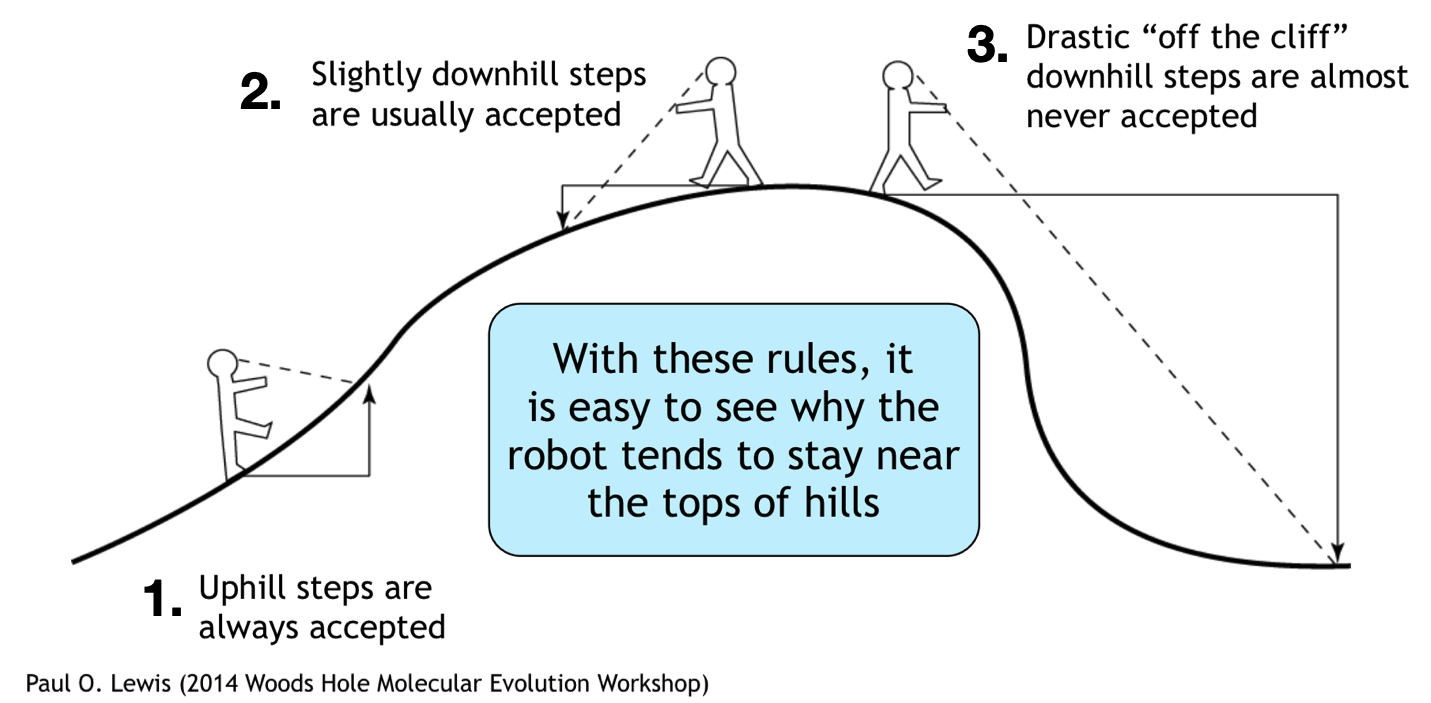
\includegraphics[height=9cm]{../graphics/mcmc-robot.png}
\end{center}

\hypertarget{mcmc-robot-rules-actual}{%
\subsection{MCMC Robot Rules (actual)}\label{mcmc-robot-rules-actual}}

\begin{center}
  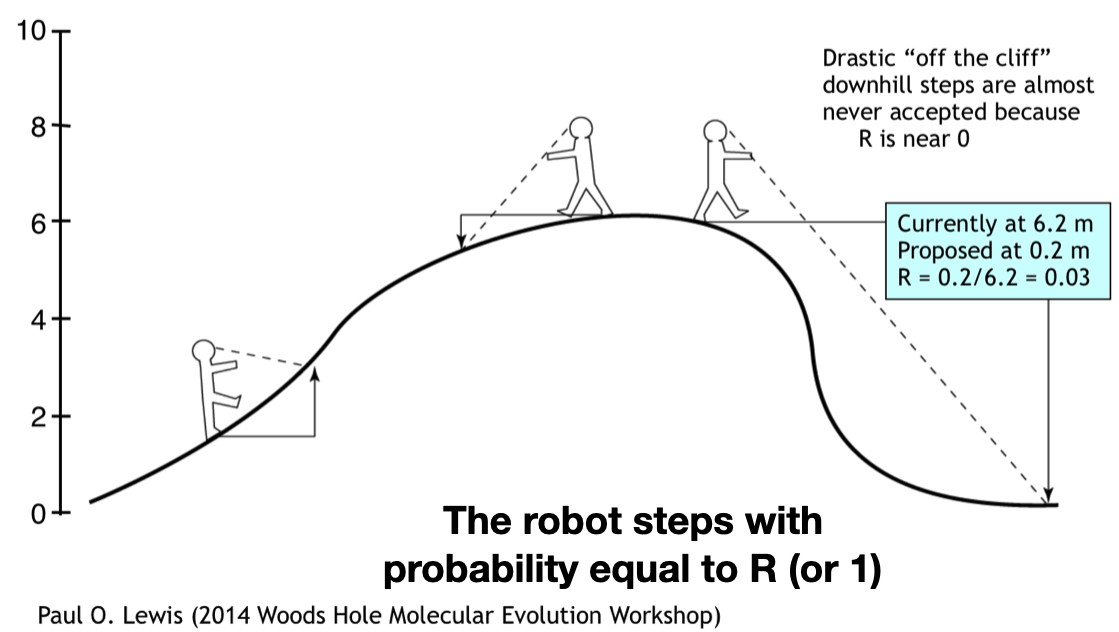
\includegraphics[height=7cm]{../graphics/mcmc-robot2.png}
\end{center}

\framebreak

\begin{center}
  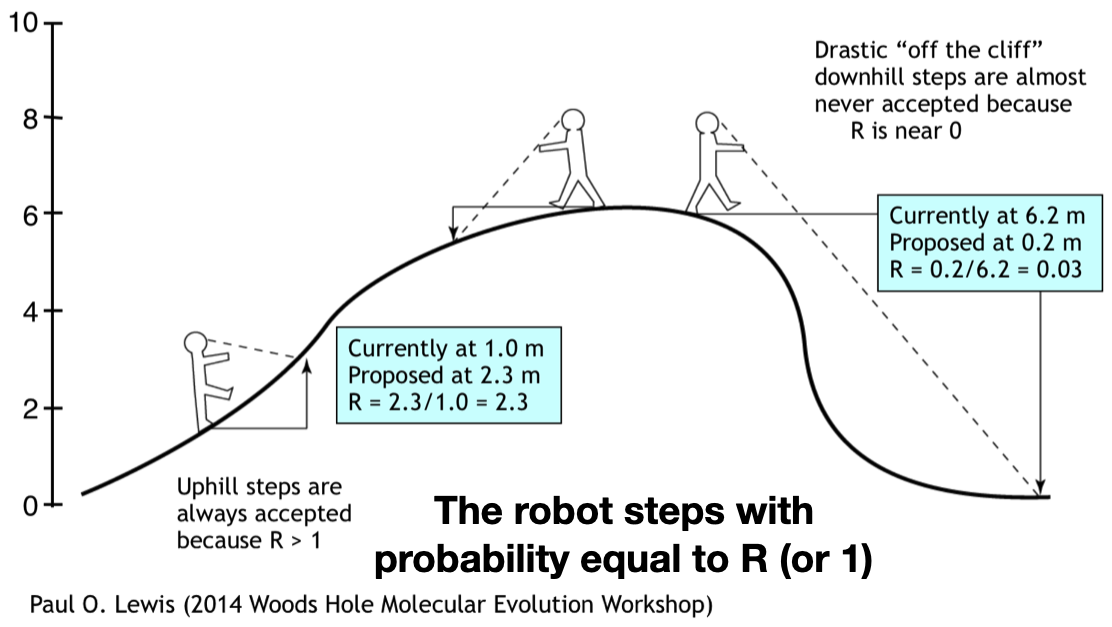
\includegraphics[height=7cm]{../graphics/mcmc-robot3.png}
\end{center}

\framebreak

\begin{center}
  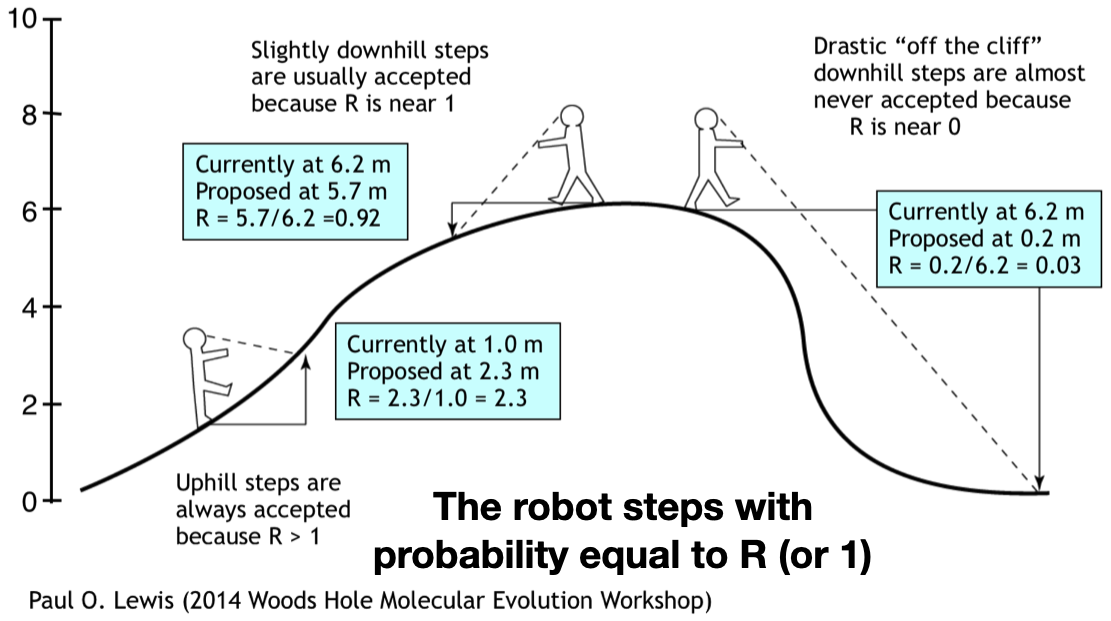
\includegraphics[height=7cm]{../graphics/mcmc-robot4.png}
\end{center}

\hypertarget{mcmc-demonstration-httpsplewis.github.ioappletsmcmc-robot}{%
\subsection{MCMC Demonstration
(https://plewis.github.io/applets/mcmc-robot/)}\label{mcmc-demonstration-httpsplewis.github.ioappletsmcmc-robot}}

\begin{center}
  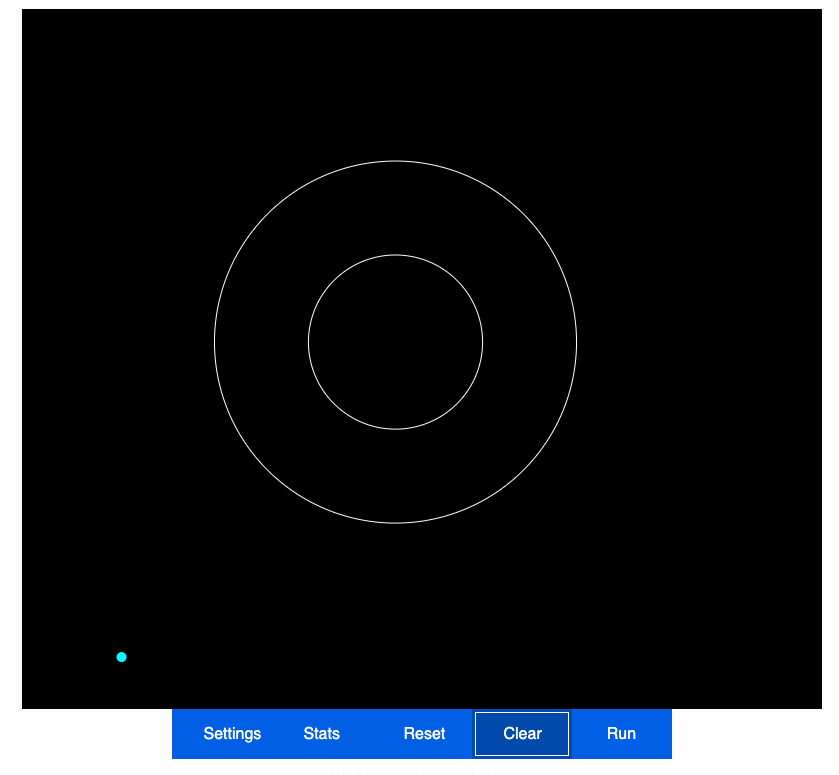
\includegraphics[height=7cm]{../graphics/mcmc-demo1.png}
\end{center}

\framebreak

\begin{center}
  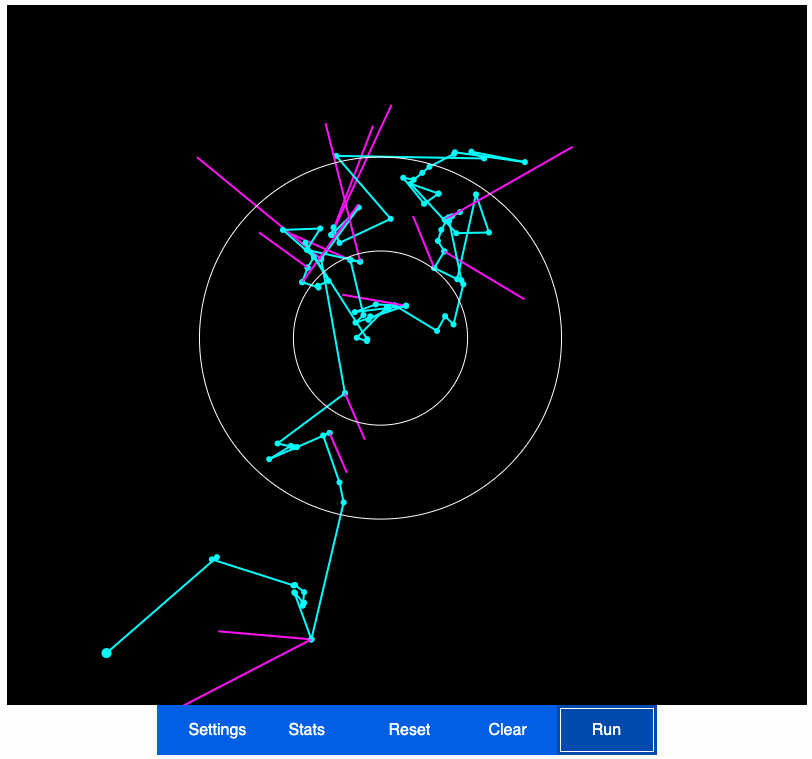
\includegraphics[height=7cm]{../graphics/mcmc-demo2.png}
\end{center}

\framebreak

\begin{center}
  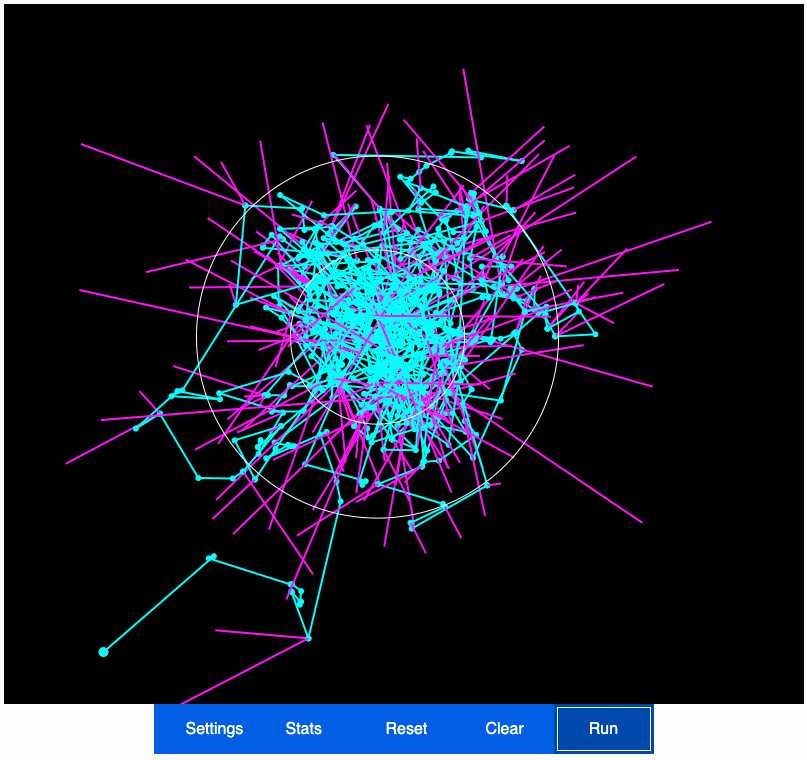
\includegraphics[height=7cm]{../graphics/mcmc-demo3.png}
\end{center}

\framebreak

\begin{center}
  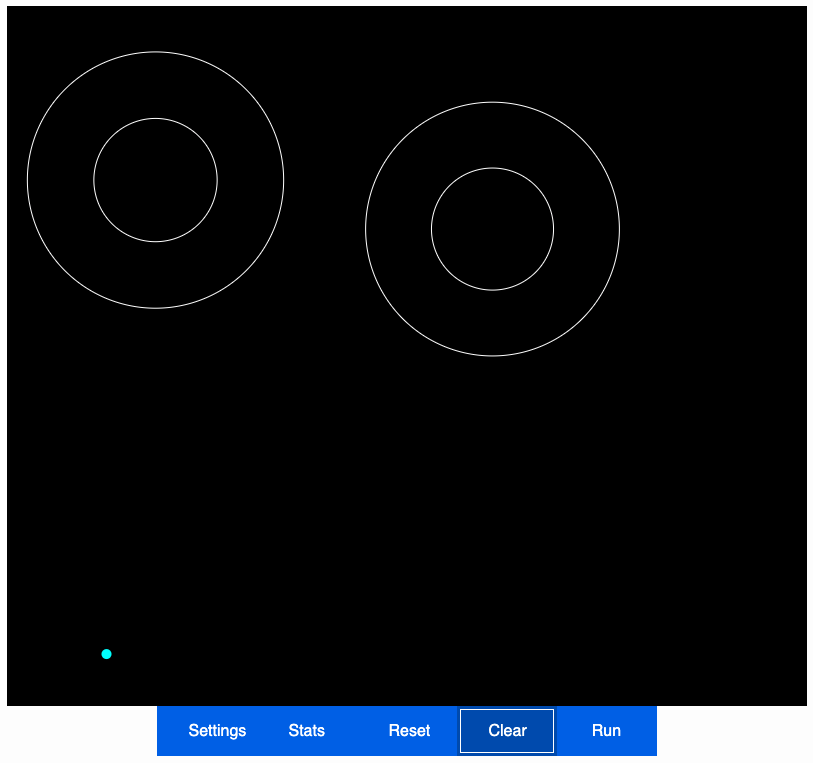
\includegraphics[height=7cm]{../graphics/mcmc-demo4.png}
\end{center}

\framebreak

\begin{center}
  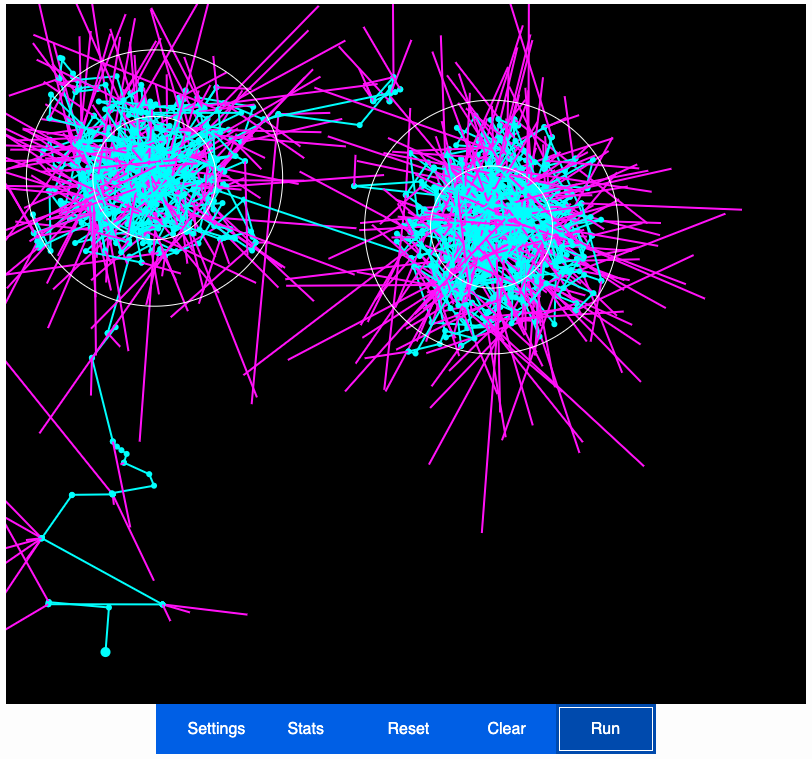
\includegraphics[height=7cm]{../graphics/mcmc-demo5.png}
\end{center}

\hypertarget{steps-for-metropolis-hastings-mcmc}{%
\subsection{Steps for Metropolis-Hastings
MCMC}\label{steps-for-metropolis-hastings-mcmc}}

\large

\begin{enumerate}
\def\labelenumi{\arabic{enumi}.}
\tightlist
\item
  Choose a reasonable starting place for parameters (\(\theta\))
\item
  Propose new parameter values (\(\theta'\))
\item
  Calculate the proposal probability \(\alpha\)
\item
  Accept (change parameters to \(\theta'\)) or reject (keep parameters
  at \(\theta\)) with probability \(\alpha\)
\item
  Repeat steps 2-5 for as many MCMC iterations as desired
\end{enumerate}

\hypertarget{steps-for-metropolis-hastings-mcmc-1}{%
\subsection{Steps for Metropolis-Hastings
MCMC}\label{steps-for-metropolis-hastings-mcmc-1}}

\large

\begin{enumerate}
\def\labelenumi{\arabic{enumi}.}
\tightlist
\item
  Choose a reasonable starting place for parameters (\(\theta\))
\item
  Propose new parameter values (\(\theta'\))
\item
  Calculate the proposal probability \(\alpha\)
\item
  Accept (change parameters to \(\theta'\)) or reject (keep parameters
  at \(\theta\))
\item
  Repeat steps 2-5 for as many MCMC iterations as desired
\end{enumerate}

Where \[\alpha = \text{min}(1, \rho)\] and
\[\rho = \frac{p(\theta'|y)}{p(\theta|y)} \cdot \frac{G(\theta|\theta')}{G(\theta'|\theta)}\]

\hypertarget{rho-equals-the-ratio-of-posterior-distributions-multiplied-by-the-proposal-probability-ratio}{%
\subsection{\texorpdfstring{\(\rho\) equals the ratio of posterior
distributions multiplied by the proposal probability
ratio}{\textbackslash rho equals the ratio of posterior distributions multiplied by the proposal probability ratio}}\label{rho-equals-the-ratio-of-posterior-distributions-multiplied-by-the-proposal-probability-ratio}}

\Huge

\[\rho = \frac{p(\theta'|y)}{p(\theta|y)} \cdot \frac{G(\theta|\theta')}{G(\theta'|\theta)}\]
\large

\begin{itemize}
\tightlist
\item
  For symmetric proposal distributions (random walks)
  \(\frac{G(\theta|\theta')}{G(\theta'|\theta)} = 1\)
\item
  Notice that the posterior denominators from before (\(p(y)\)) cancel
  each other out in this ratio
\end{itemize}

\hypertarget{we-can-simplify-the-acceptance-probability-significantly}{%
\subsection{We can simplify the acceptance probability
significantly}\label{we-can-simplify-the-acceptance-probability-significantly}}

\Huge

\[\rho = \frac{p(y|\theta')p(\theta')}{p(y|\theta)p(\theta)}\] \Large

\begin{itemize}
\tightlist
\item
  Only depends on the likelihood and prior probabilities
\end{itemize}

\hypertarget{prior-parameter-distributions}{%
\subsection{Prior parameter
distributions}\label{prior-parameter-distributions}}

\Large

\begin{itemize}
\tightlist
\item
  Prior distributions assign probabilities to specific parameter values
  and are created separately for every parameter
\item
  Other than strict constraints, we expect the data and likelihood to
  drive the posterior distribution, but always good idea to check the
  impact the prior distributions have in a sensitivity analysis
\end{itemize}

\hypertarget{three-main-types-of-prior-distributions}{%
\subsection{Three main types of prior
distributions}\label{three-main-types-of-prior-distributions}}

\Large

\begin{enumerate}
\def\labelenumi{\arabic{enumi}.}
\tightlist
\item
  Informative priors craft a distribution based on previous scientific
  studies

  \begin{itemize}
  \tightlist
  \item
    Typically only used if a specific quantity is well known from
    outside data (e.g.~the infection fatality rate or infectious period)
  \end{itemize}
\item
  Weakly informative priors craft a distribution with reasonable
  constraints

  \begin{itemize}
  \tightlist
  \item
    Used for regularization (e.g.~to ``suggest'' that a parameter is
    most likely to be positive)
  \end{itemize}
\item
  Uninformative (flat priors) assign equal probabilities across a range
  of plausible values

  \begin{itemize}
  \tightlist
  \item
    Can constrain parameters to be strictly positive or in
    biologically/epidemiologically relevant range
  \item
    Not always ``uninformative''
  \end{itemize}
\end{enumerate}

\hypertarget{questions-about-mcmc}{%
\subsection{Questions about MCMC?}\label{questions-about-mcmc}}

\hypertarget{pmcmc}{%
\subsection{PMCMC}\label{pmcmc}}

\Huge

\[p(y|\theta)p(\theta)\]

\large

\begin{itemize}
\tightlist
\item
  Standard MCMC algorithm assumes a deterministic likelihood
\item
  When process stochasticisty is included we use the particle filter to
  obtain likelihood
\item
  Particle filter (Sequential Monte Carlo procedure) approximates
  \(p(y|\theta)\), but with variability

  \begin{itemize}
  \tightlist
  \item
    Can complicate things a bit, but usually not an issue
  \end{itemize}
\end{itemize}

\hypertarget{further-pmcmc-resources}{%
\subsection{Further PMCMC resources}\label{further-pmcmc-resources}}

\large

\begin{itemize}
\tightlist
\item
  For an awesome field-specific explanation

  \begin{itemize}
  \tightlist
  \item
    \href{https://doi.org/10.1016/j.epidem.2019.100363}{Introduction to
    particle Markov-chain Monte Carlo for disease dynamics modellers}
  \end{itemize}
\item
  For some considerations with modeling and inference

  \begin{itemize}
  \tightlist
  \item
    \href{https://www.sciencedirect.com/science/article/pii/S1755436519300441}{Choices
    and trade-offs in inference with infectious disease models}
  \end{itemize}
\item
  For an example of how it has been used in recent epidemiological
  literature

  \begin{itemize}
  \tightlist
  \item
    \href{https://www.medrxiv.org/content/10.1101/2024.01.10.24301116v1}{Estimating
    SARS-CoV-2 transmission parameters between coinciding outbreaks in a
    university population and the surrounding community}
  \end{itemize}
\item
  For working with pmcmc in the \texttt{pomp} package

  \begin{itemize}
  \tightlist
  \item
    \href{https://kingaa.github.io/pomp/vignettes/getting_started.html\#Sampling_the_posterior_using_particle_Markov_chain_Monte_Carlo}{Getting
    started with pomp}
  \end{itemize}
\end{itemize}

\hypertarget{considerations-for-moving-from-mif2-to-pmcmc-in-pomp}{%
\subsection{\texorpdfstring{Considerations for moving from \texttt{mif2}
to \texttt{pmcmc} in
\texttt{pomp}}{Considerations for moving from mif2 to pmcmc in pomp}}\label{considerations-for-moving-from-mif2-to-pmcmc-in-pomp}}

\Large

\begin{enumerate}
\def\labelenumi{\arabic{enumi}.}
\tightlist
\item
  Specify the prior distributions for all parameters
\item
  Use the \texttt{pmcmc()} function
\item
  Use MCMC diagnostics to check convergence, etc.
\end{enumerate}

\hypertarget{influenza-boarding-school-example}{%
\subsection{Influenza boarding school
example}\label{influenza-boarding-school-example}}

\large

\begin{itemize}
\tightlist
\item
  1978 influenza epidemic in boarding school that infected much of the
  school
\item
  Data are actually kids in beds, but we are assuming it's new
  infections
\end{itemize}

\begin{figure}[h!]

{\centering 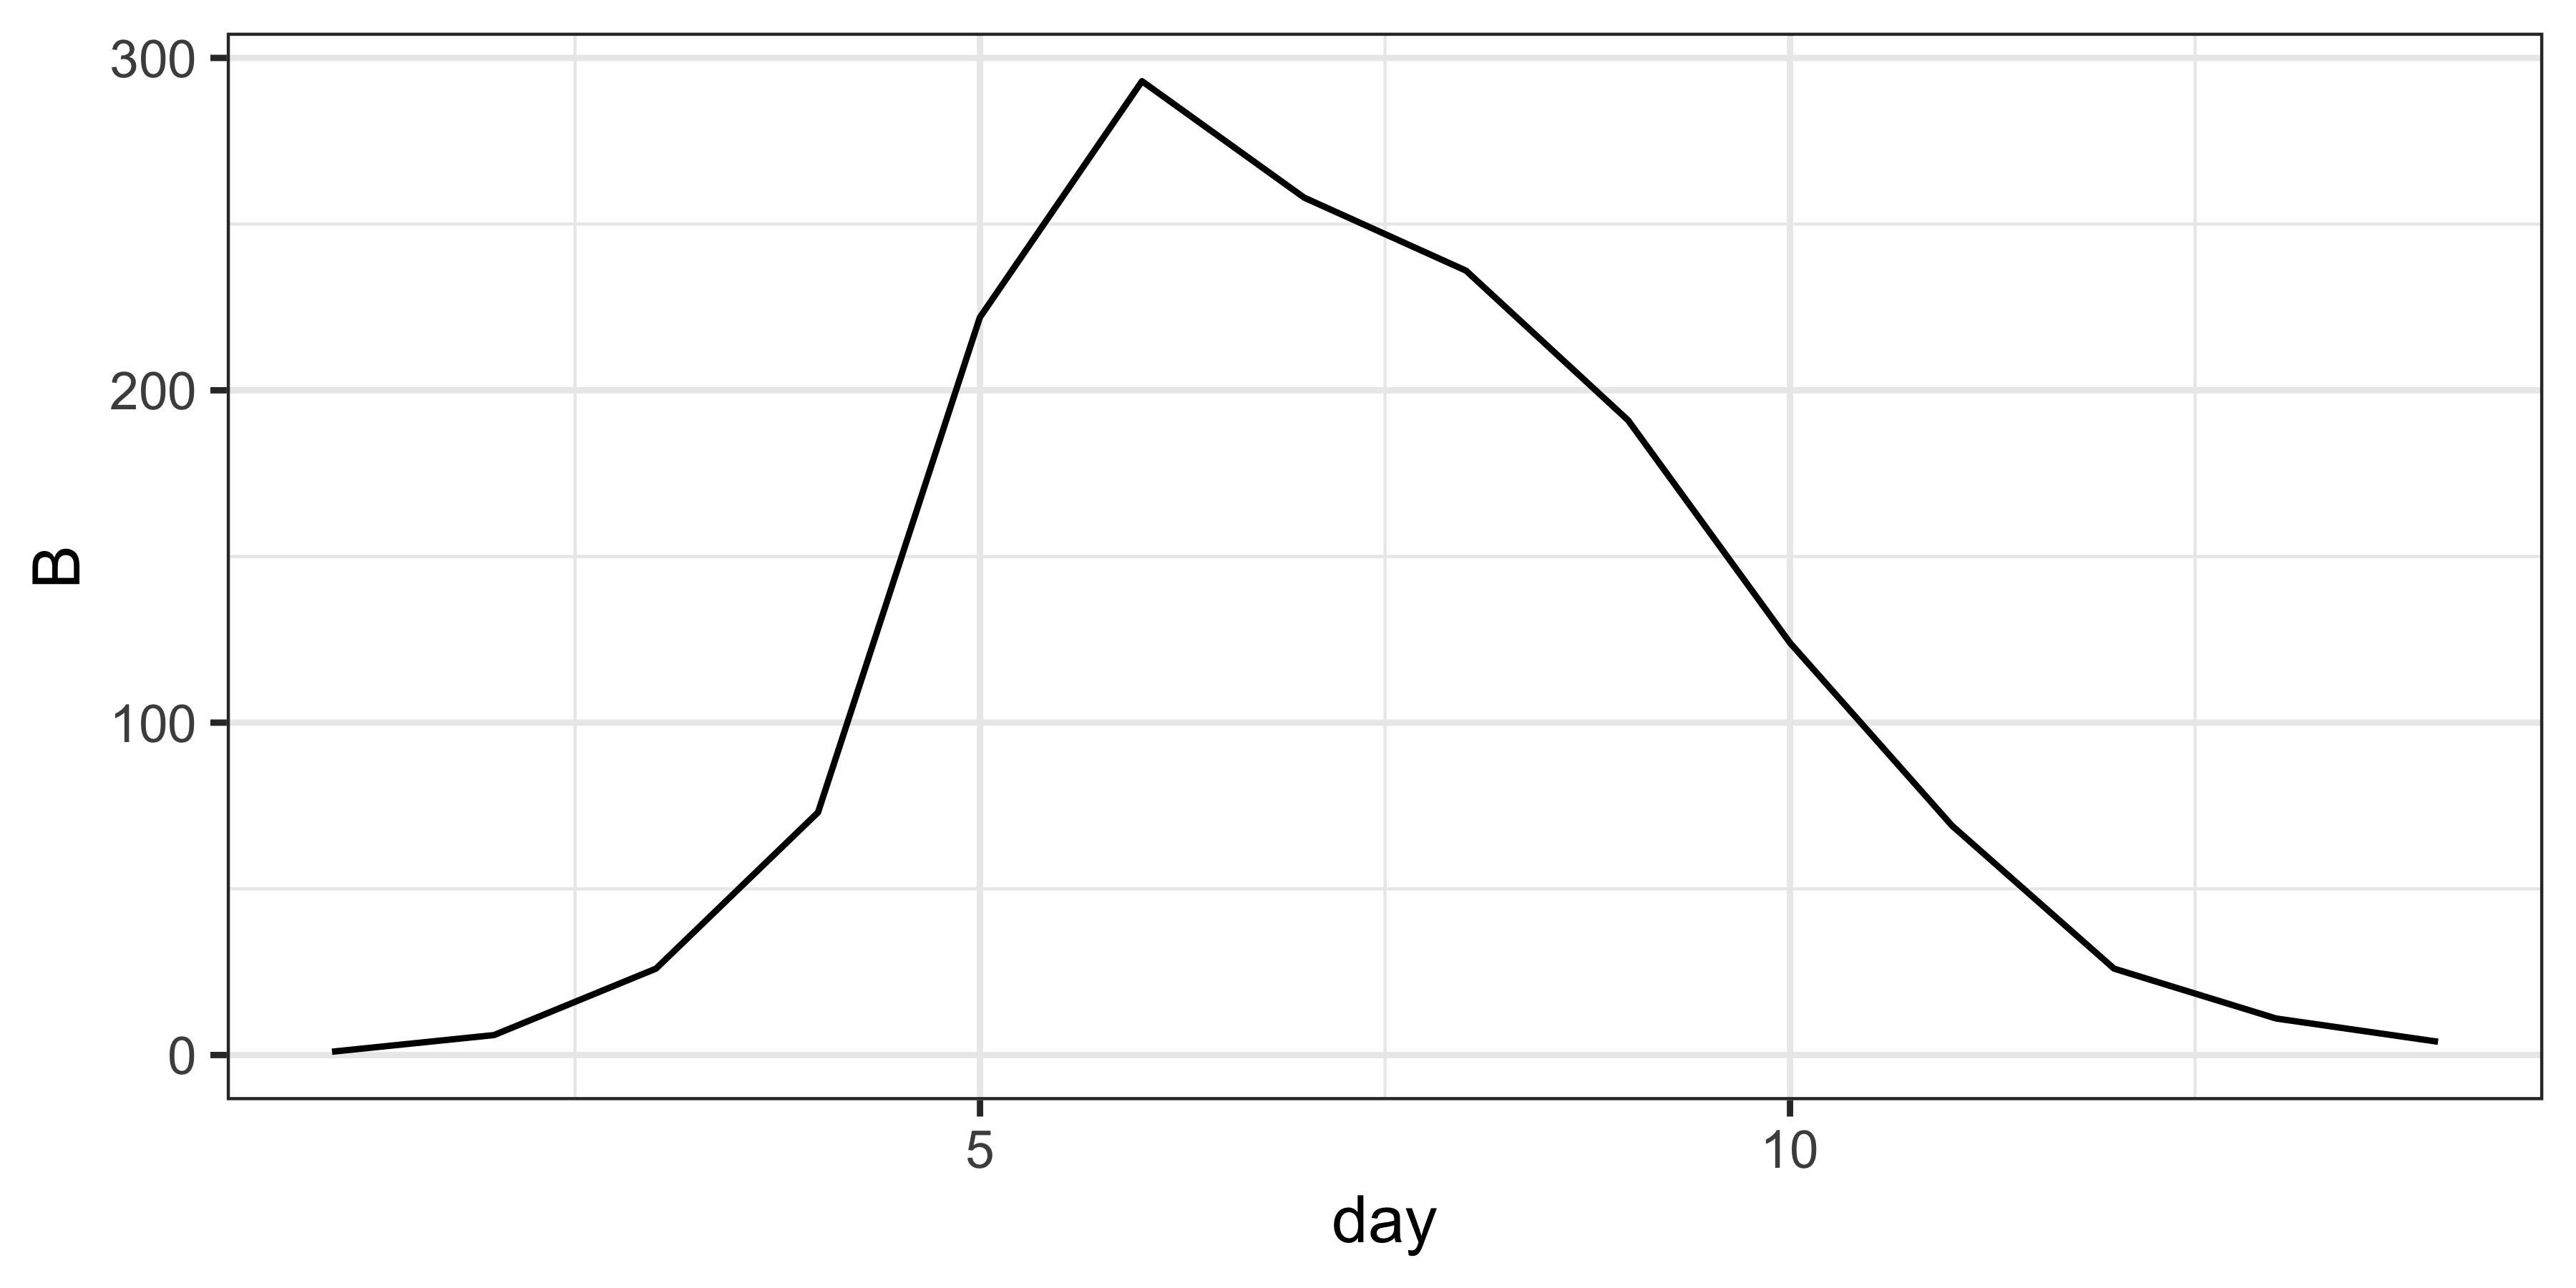
\includegraphics[width=\textwidth,height=0.6\textheight]{tmp//figure/boardingplot-1.png}

}

\end{figure}

\hypertarget{modeling-as-an-sir-model-with-reporting-of-new-infections}{%
\subsection{Modeling as an SIR model with reporting of new
infections}\label{modeling-as-an-sir-model-with-reporting-of-new-infections}}

\begin{center}
  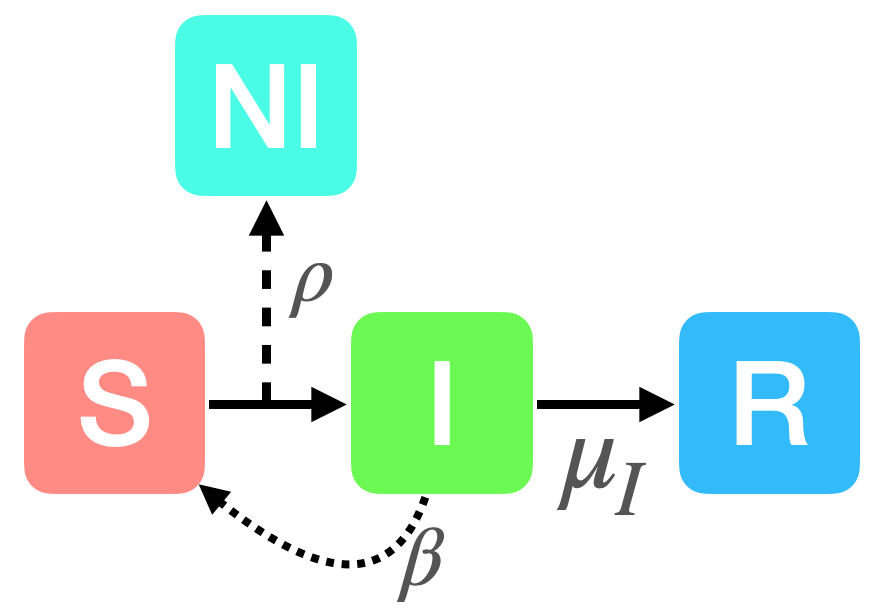
\includegraphics[height=6cm]{../graphics/boarding-school-model.png}
\end{center}

\hypertarget{modeling-as-an-sir-model-with-reporting-of-new-infections-1}{%
\subsection{Modeling as an SIR model with reporting of new
infections}\label{modeling-as-an-sir-model-with-reporting-of-new-infections-1}}

\begin{Shaded}
\begin{Highlighting}[]
\NormalTok{rproc }\OtherTok{\textless{}{-}} \FunctionTok{Csnippet}\NormalTok{(}\StringTok{"}
\StringTok{  double N = 2000;}
\StringTok{  double t1 = rbinom(S,1{-}exp({-}Beta*I/N*dt));}
\StringTok{  double t2 = rbinom(I,1{-}exp({-}mu\_I*dt));}
\StringTok{  S  {-}= t1;}
\StringTok{  I  += t1 {-} t2;}
\StringTok{  NI += t1;}
\StringTok{  R += t2;}
\StringTok{"}\NormalTok{)}

\NormalTok{rmeas }\OtherTok{\textless{}{-}} \FunctionTok{Csnippet}\NormalTok{(}\StringTok{"}
\StringTok{  B = rpois(rho*NI+1e{-}6);}
\StringTok{"}\NormalTok{)}
\end{Highlighting}
\end{Shaded}

\hypertarget{specifying-the-prior-distribution}{%
\subsection{Specifying the prior
distribution}\label{specifying-the-prior-distribution}}

\begin{Shaded}
\begin{Highlighting}[]
\NormalTok{priorDens }\OtherTok{\textless{}{-}} \FunctionTok{Csnippet}\NormalTok{(}\StringTok{"}
\StringTok{  lik = dunif(Beta, 1, 4, 1) +}
\StringTok{        dunif(mu\_I, 0.5, 3, 1) +}
\StringTok{        dunif(rho, 0.5, 1, 1);}
\StringTok{  if (!give\_log) lik = exp(lik);}
\StringTok{"}\NormalTok{)}
\end{Highlighting}
\end{Shaded}

\large

\begin{itemize}
\tightlist
\item
  Add the densities (probabilities) for each parameter value
  independently
\item
  Include the same log functionality used before
\item
  We are specifying a plausible range of values for each parameter here
\end{itemize}

\hypertarget{running-an-mcmc-chain}{%
\subsection{Running an MCMC chain}\label{running-an-mcmc-chain}}

\begin{Shaded}
\begin{Highlighting}[]
\NormalTok{flu }\SpecialCharTok{|\textgreater{}} \DocumentationTok{\#\# Standard pomp object that has already been created }
  \FunctionTok{pomp}\NormalTok{(}\AttributeTok{dprior =}\NormalTok{ priorDens, }\DocumentationTok{\#\# Prior specified from previous slide}
       \AttributeTok{params =}\NormalTok{ sim\_params, }\DocumentationTok{\#\# Parameter starting point}
       \AttributeTok{paramnames=}\FunctionTok{c}\NormalTok{(}\StringTok{"Beta"}\NormalTok{,}\StringTok{"mu\_I"}\NormalTok{,}\StringTok{"rho"}\NormalTok{)) }\SpecialCharTok{|\textgreater{}} \DocumentationTok{\#\# Parameter names}
  \FunctionTok{pmcmc}\NormalTok{(}\AttributeTok{Nmcmc =} \DecValTok{10000}\NormalTok{, }\DocumentationTok{\#\# Number of MCMC iterations}
        \AttributeTok{Np =} \DecValTok{200}\NormalTok{, }\DocumentationTok{\#\# Number of particles to use}
        \AttributeTok{proposal =} \FunctionTok{mvn\_diag\_rw}\NormalTok{(}\AttributeTok{rw.sd =} \FunctionTok{c}\NormalTok{(}\AttributeTok{Beta=}\FloatTok{0.3}\NormalTok{, }\AttributeTok{mu\_I=}\FloatTok{0.3}\NormalTok{, }\AttributeTok{rho=}\FloatTok{0.1}\NormalTok{))}
\NormalTok{  ) }\OtherTok{{-}\textgreater{}}\NormalTok{ test\_mcmc}
\end{Highlighting}
\end{Shaded}

\hypertarget{proposal-distributions-in-pomp}{%
\subsection{\texorpdfstring{Proposal distributions in
\texttt{pomp}}{Proposal distributions in pomp}}\label{proposal-distributions-in-pomp}}

\Large

\begin{itemize}
\tightlist
\item
  \texttt{mvn\_diag\_rw(rw.sd)} - you provide the standard deviations
  for the proposals for each parameter
\item
  \texttt{mvn\_rw(rw.var)} - you provide the variance/covariance matrix
  for proposals
\item
  \texttt{mvn\_rw\_adaptive()} - you provide either of the above and it
  attempts to automatically ``tune'' parameters to achieve good MCMC
  mixing
\end{itemize}

\hypertarget{typically-you-need-to-test-different-values-initially}{%
\subsection{Typically you need to test different values
initially}\label{typically-you-need-to-test-different-values-initially}}

\begin{Shaded}
\begin{Highlighting}[]
\NormalTok{flu }\SpecialCharTok{|\textgreater{}} \DocumentationTok{\#\# Standard pomp object that has already been created }
  \FunctionTok{pomp}\NormalTok{(}\AttributeTok{dprior =}\NormalTok{ priorDens, }\DocumentationTok{\#\# Prior specified from previous slide}
       \AttributeTok{params =}\NormalTok{ sim\_params, }\DocumentationTok{\#\# Parameter starting point}
       \AttributeTok{paramnames=}\FunctionTok{c}\NormalTok{(}\StringTok{"Beta"}\NormalTok{,}\StringTok{"mu\_I"}\NormalTok{,}\StringTok{"rho"}\NormalTok{)) }\SpecialCharTok{|\textgreater{}} \DocumentationTok{\#\# Parameter names}
  \FunctionTok{pmcmc}\NormalTok{(}\AttributeTok{Nmcmc =} \DecValTok{10000}\NormalTok{, }\DocumentationTok{\#\# Number of MCMC iterations}
        \AttributeTok{Np =} \DecValTok{200}\NormalTok{, }\DocumentationTok{\#\# Number of particles to use}
        \AttributeTok{proposal =} \FunctionTok{mvn\_diag\_rw}\NormalTok{(}\AttributeTok{rw.sd =} \FunctionTok{c}\NormalTok{(}\AttributeTok{Beta=}\FloatTok{0.3}\NormalTok{, }\AttributeTok{mu\_I=}\FloatTok{0.3}\NormalTok{, }\AttributeTok{rho=}\FloatTok{0.1}\NormalTok{))}
\NormalTok{  ) }\OtherTok{{-}\textgreater{}}\NormalTok{ test\_mcmc}
\end{Highlighting}
\end{Shaded}

\hypertarget{diagnosing-chain-mixing}{%
\subsection{Diagnosing chain mixing}\label{diagnosing-chain-mixing}}

\begin{center}
  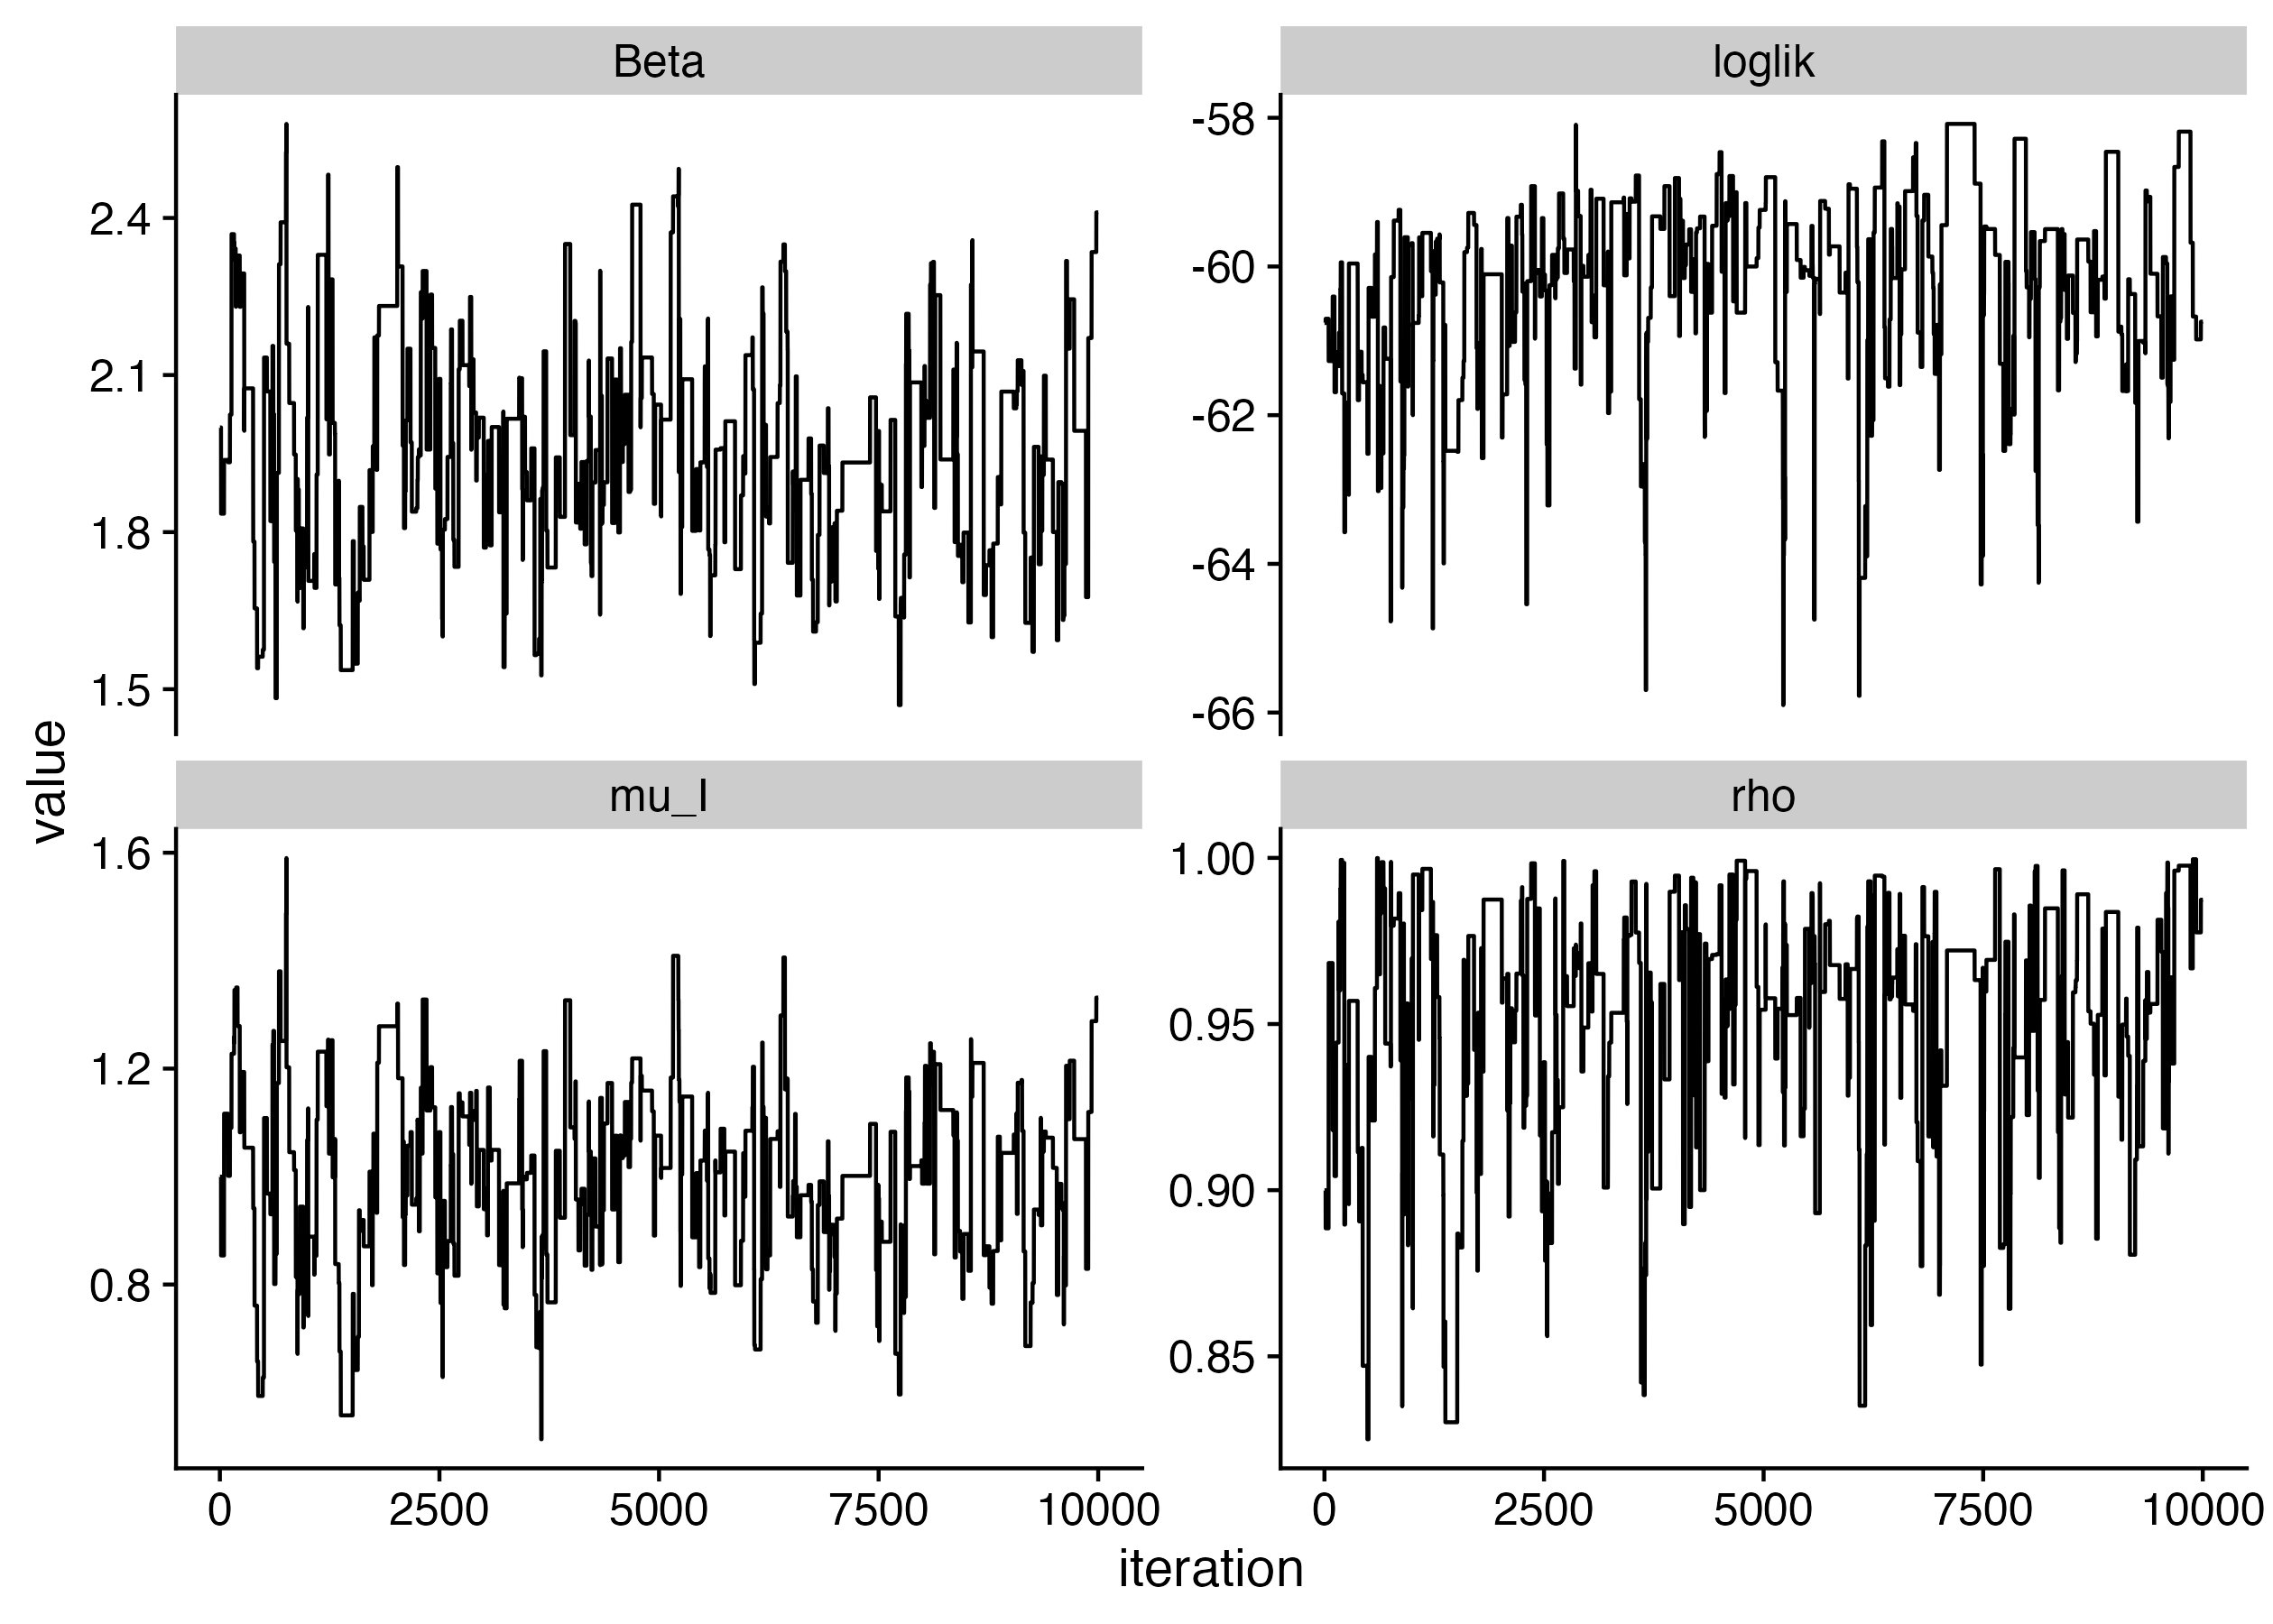
\includegraphics[height=8cm]{../graphics/test-mcmc-trace.png}
\end{center}

\hypertarget{diagnosing-chain-mixing---autocorrelation}{%
\subsection{Diagnosing chain mixing -
autocorrelation}\label{diagnosing-chain-mixing---autocorrelation}}

\begin{Shaded}
\begin{Highlighting}[]
\FunctionTok{library}\NormalTok{(coda)}

\NormalTok{test\_mcmc }\SpecialCharTok{|\textgreater{}} 
  \FunctionTok{traces}\NormalTok{() }\SpecialCharTok{|\textgreater{}}  
  \FunctionTok{autocorr.diag}\NormalTok{(}\AttributeTok{lags=}\FunctionTok{c}\NormalTok{(}\DecValTok{10}\NormalTok{, }\DecValTok{50}\NormalTok{, }\DecValTok{100}\NormalTok{))}
\end{Highlighting}
\end{Shaded}

\begin{verbatim}
           loglik log.prior      Beta      mu_I       rho
Lag 10  0.8603731 0.9990001 0.8845398 0.8810328 0.8023407
Lag 50  0.5396487 0.9950005 0.5445343 0.5645781 0.3971658
Lag 100 0.3494610 0.9900010 0.3271410 0.3358897 0.2386606
            mu_R1
Lag 10  0.9990001
Lag 50  0.9950005
Lag 100 0.9900010
\end{verbatim}

\hypertarget{second-step-often-uses-the-empirical-covariance-matrix-for-proposals-to-improve-mixing}{%
\subsection{Second step often uses the empirical covariance matrix for
proposals to improve
mixing}\label{second-step-often-uses-the-empirical-covariance-matrix-for-proposals-to-improve-mixing}}

\begin{Shaded}
\begin{Highlighting}[]
\NormalTok{flu }\SpecialCharTok{|\textgreater{}} 
  \FunctionTok{pomp}\NormalTok{(}\AttributeTok{dprior =}\NormalTok{ priorDens,}
       \AttributeTok{params =}\NormalTok{ sim\_params, }\DocumentationTok{\#\#Using the sim params as a starting spot}
       \AttributeTok{paramnames=}\FunctionTok{c}\NormalTok{(}\StringTok{"Beta"}\NormalTok{,}\StringTok{"mu\_I"}\NormalTok{,}\StringTok{"rho"}\NormalTok{)) }\SpecialCharTok{|\textgreater{}} 
  \FunctionTok{pmcmc}\NormalTok{(}\AttributeTok{Nmcmc =} \DecValTok{10000}\NormalTok{, }
        \AttributeTok{Np =} \DecValTok{200}\NormalTok{,}
        \AttributeTok{proposal =} \FunctionTok{mvn\_rw}\NormalTok{(}\FunctionTok{covmat}\NormalTok{(test\_mcmc, }\AttributeTok{thin =} \DecValTok{50}\NormalTok{))}
\NormalTok{  ) }\OtherTok{{-}\textgreater{}}\NormalTok{ test\_mcmc2}
\end{Highlighting}
\end{Shaded}

\hypertarget{improved-trace-plots}{%
\subsection{Improved trace plots!}\label{improved-trace-plots}}

\begin{center}
  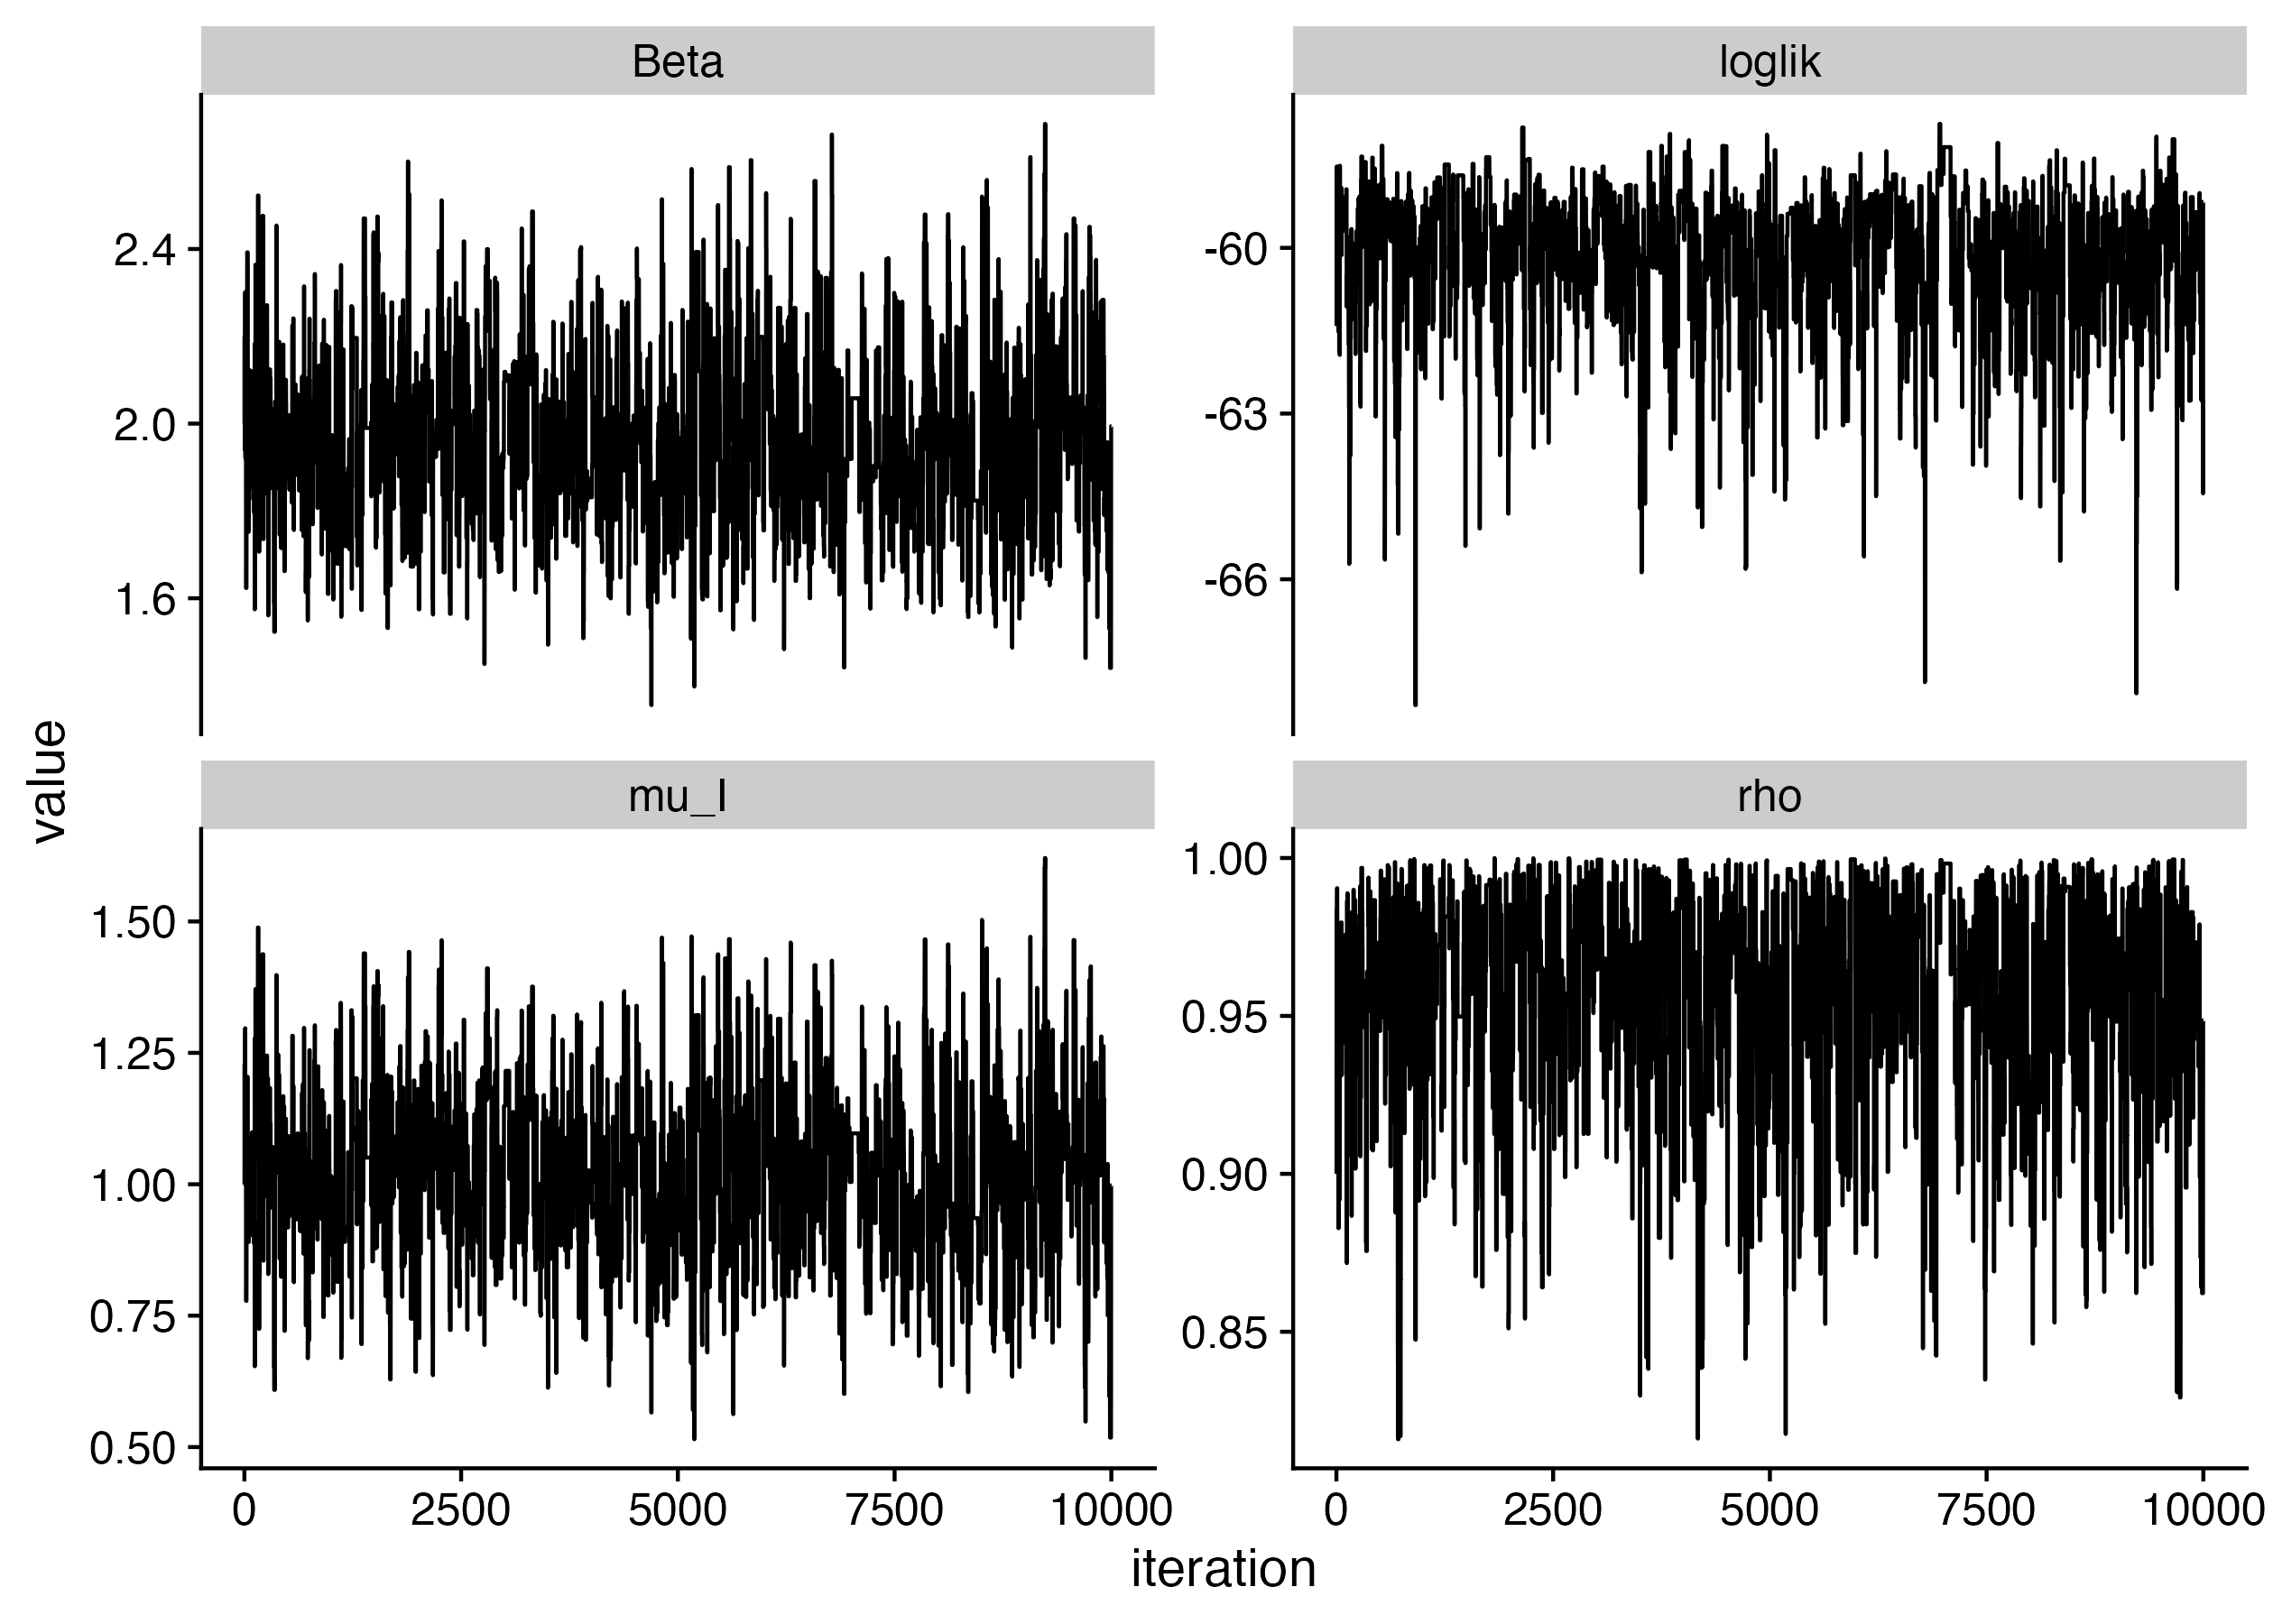
\includegraphics[height=8cm]{../graphics/test-mcmc-trace2.png}
\end{center}

\hypertarget{improved-autocorrelation}{%
\subsection{Improved autocorrelation!}\label{improved-autocorrelation}}

\begin{Shaded}
\begin{Highlighting}[]
\NormalTok{test\_mcmc2 }\SpecialCharTok{|\textgreater{}} 
  \FunctionTok{traces}\NormalTok{() }\SpecialCharTok{|\textgreater{}}  
  \FunctionTok{autocorr.diag}\NormalTok{(}\AttributeTok{lags=}\FunctionTok{c}\NormalTok{(}\DecValTok{10}\NormalTok{, }\DecValTok{50}\NormalTok{, }\DecValTok{100}\NormalTok{))}
\end{Highlighting}
\end{Shaded}

\begin{verbatim}
            loglik log.prior         Beta        mu_I
Lag 10  0.37014612 0.9990001  0.309750841  0.32244825
Lag 50  0.02823492 0.9950005 -0.057939058 -0.03009082
Lag 100 0.01502889 0.9900010 -0.005065156 -0.02058864
                rho     mu_R1
Lag 10   0.30978973 0.9990001
Lag 50  -0.01285783 0.9950005
Lag 100 -0.02784212 0.9900010
\end{verbatim}

\hypertarget{estimating-posterior-distributions}{%
\subsection{Estimating posterior
distributions}\label{estimating-posterior-distributions}}

\large

\begin{enumerate}
\def\labelenumi{\arabic{enumi}.}
\tightlist
\item
  Once you are happy with the mixing of your \texttt{pmcmc} you are
  ready to do a run for estimating posteriors
\item
  First randomly choose 3-5 starting parameter values (example uses
  Latin-hypercube sampling)
\item
  Run (in parallel or not depending on computational time) a chain
  intialized with each
\item
  Diagnose chain mixing with trace plots and Gelman-Rubin convergence
  diagnostic
\item
  Remove the burn-in period and thin based on diagnostics
\item
  Summarize parameter posterior distributions and credible intervals
\end{enumerate}

\hypertarget{summary-process-for-pmcmc-in-pomp}{%
\subsection{\texorpdfstring{Summary process for PMCMC in
\texttt{pomp}}{Summary process for PMCMC in pomp}}\label{summary-process-for-pmcmc-in-pomp}}

\large

\begin{enumerate}
\def\labelenumi{\arabic{enumi}.}
\tightlist
\item
  Create \texttt{pomp} object exactly as normal
\item
  Create the prior distributions for parameters
\item
  Run an initial \texttt{pmcmc} with \texttt{mvn\_diag\_rw} proposal to
  make sure it's working and diagnose
\item
  Randomly sample 3-5 parameter starting conditions
\item
  Run a PMCMC chain with \texttt{mvn\_rw()} proposal and the
  variance/covariance matrix from the first run for each of the initial
  parameter combinations
\item
  Diagnose mixing and convergence (alter components as needed)
\item
  Summarize parameters
\end{enumerate}

\hypertarget{activity-how-do-stochastic-and-deterministic-models-differ}{%
\subsection{Activity: how do stochastic and deterministic models
differ?}\label{activity-how-do-stochastic-and-deterministic-models-differ}}

\Large

\begin{enumerate}
\def\labelenumi{\arabic{enumi}.}
\tightlist
\item
  Go to https://plewis.github.io/applets/mcmc-robot/, and play with
  different MCMC parameters and variations
\item
  Download the exercise code for the influenza boarding school example
  and test the impact of the following on mixing and traceplots:

  \begin{itemize}
  \tightlist
  \item
    Different parameters for the proposal distribution
  \item
    Different starting parameter values
  \item
    Different number of particles
  \end{itemize}
\end{enumerate}

\hypertarget{license-acknowledgments-and-links}{%
\subsection{License, acknowledgments, and
links}\label{license-acknowledgments-and-links}}

\begin{itemize}
\item
  This lesson is prepared for the
  \href{https://rubbislam.quarto.pub/episim/}{Simulation-based Inference
  for Epidemiological Dynamics} module at the Summer Institute in
  Statistics and Modeling in Infectious Diseases,
  \href{https://sph.emory.edu/SISMID/index.html}{SISMID}.
\item
  The materials build on \href{../acknowledge.html}{previous versions of
  this course and related courses}.
\item
  Licensed under the
  \href{https://creativecommons.org/licenses/by-nc/4.0/}{Creative
  Commons Attribution-NonCommercial license}. Please share and remix
  non-commercially, mentioning its origin.
  
\includegraphics[height=12pt]{../graphics/cc-by-nc}
\item
  Produced with R version 4.3.2 and pomp version 5.10.
\item
  Compiled on 2024-07-24.
\end{itemize}

\vfill

\href{index.html}{Back to Lesson}

\href{./main.R}{\texttt{R} code for this lesson}



\end{document}
